\documentclass[tikz,convert={density=300, outfile=\jobname.png}]{standalone}
\usepackage[utf8]{inputenc}
\usepackage{tikz}

\usetikzlibrary{calc}

\usetikzlibrary{shapes.geometric}
\usetikzlibrary{positioning}

\begin{document}
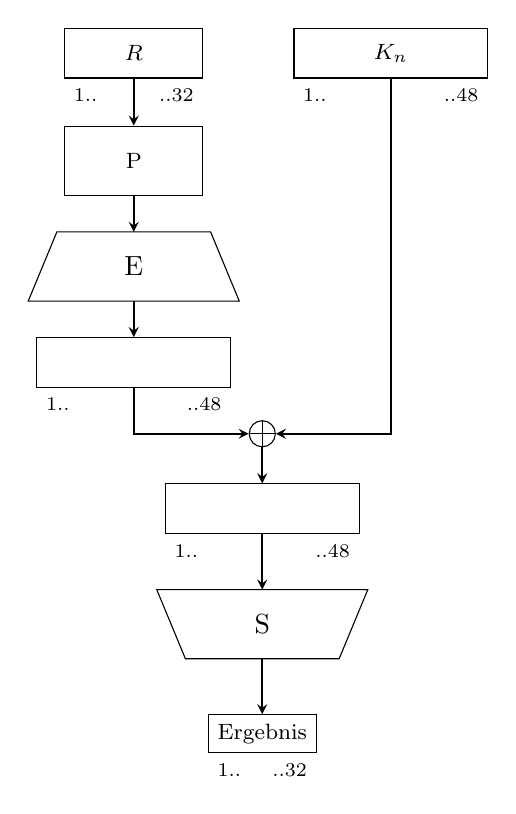
\begin{tikzpicture}



\tikzset{half paths/.style 2 args={%
  decoration={show path construction,
    lineto code={
      \draw [#1] (\tikzinputsegmentfirst) -- 
         ($(\tikzinputsegmentfirst)!0.5!(\tikzinputsegmentlast)$);
      \draw [#2] ($(\tikzinputsegmentfirst)!0.5!(\tikzinputsegmentlast)$)
        -- (\tikzinputsegmentlast);
    }
  }, decorate
}}

\tikzset{
	smallarrow/.style={-{stealth[width=1pt]}}
}

\tikzset{
    myarrow/.style={-{stealth}, semithick},
    myline/.style={semithick},
    triangle/.style = {draw, regular polygon, regular polygon sides=3, inner sep=0pt, minimum height=130},
    node rotated/.style = {rotate=180},
    border rotated/.style = {shape border rotate=180},
     pre/.style={<-,shorten <=1pt,>=stealth',semithick},
     post/.style={->,shorten >=1pt,>=stealth',semithick}
}

\tikzset{XOR/.style={draw,circle,append after command={
        [shorten >=\pgflinewidth, shorten <=\pgflinewidth, semithick,]
        (\tikzlastnode.north) edge (\tikzlastnode.south)
        (\tikzlastnode.east) edge (\tikzlastnode.west)
        }
    }
}

\pgfmathsetmacro{\L}{70}
\pgfmathsetmacro{\S}{50}

\tikzset{
	trapez/.style={
	trapezium, trapezium angle=67.5, draw,inner xsep=0pt,outer sep=0pt,
	minimum height=25pt, text width=#1
	}
}

%%%%%%%%%%%%%%%%%%%%%%%%%%%%%%%%%%%%%%%%%%%%%%%%%%%%%%%%%
%                       Begin Picture                   %
%%%%%%%%%%%%%%%%%%%%%%%%%%%%%%%%%%%%%%%%%%%%%%%%%%%%%%%%%

%middle empty node
\node[draw, minimum width=\L pt, minimum height=18] (res) {};
\node[below=6pt of res.south west, anchor=west] () {\scriptsize 1..};
\node[below=6pt of res.south east, anchor=east] () {\scriptsize ..48};


%xor point
\node[XOR, above=13pt of res.north] (x) {};
\draw[myarrow] (x) -- (res.north);

%S
\node[trapez=\S - 20, below=20pt of res.south, shape border rotate=180, align=center] (S) {S};
\draw[myarrow] (res.south) -- (S.north);

%ergebnis
\node[draw, below=20pt of S.south] (retval) {\footnotesize Ergebnis};
\node[below=6pt of retval.south west, anchor=west] () {\scriptsize 1..};
\node[below=6pt of retval.south east, anchor=east] () {\scriptsize ..32};
\draw[myarrow] (S.south) -- (retval.north);

%left branch
\node[left=\L / 2 + 3pt of x] (anchl) {};

%in between empty node
\node[draw, minimum width=\L pt, minimum height=18, above=13pt of anchl] (leftempty) {};
\node[below=6pt of leftempty.south west, anchor=west] () {\scriptsize 1..};
\node[below=6pt of leftempty.south east, anchor=east] () {\scriptsize ..48};

%E
\node[trapez=\S - 20, above=13pt of leftempty, align=center] (E) {E};
\draw[myarrow] (leftempty.south) -- (anchl.center) -- (x.west);
\draw[myarrow] (E.south) -- (leftempty.north);

%P
\node[draw, above=13pt of E.north, minimum width=\S pt, minimum height=25pt] (P) {\footnotesize P};

\draw[myarrow] (P.south) -- (E.north);

\node[draw, above=17pt of P.north, minimum width=\S pt, minimum height=18] (R) {\footnotesize $R$};
\node[below=6pt of R.south west, anchor=west] () {\scriptsize 1..};
\node[below=6pt of R.south east, anchor=east] () {\scriptsize ..32};
\draw[myarrow] (R.south) -- (P.north);


%right branch
\node[right=\L / 2 + 3pt of x] (anchr) {};

\path
  let \p0 = (anchr),
      \p1 = (R)
  in
node [draw, , minimum width=\L pt, minimum height=18] (K) at (\x0, \y1) {\footnotesize $K_{n}$};
\node[below=6pt of K.south west, anchor=west] () {\scriptsize 1..};
\node[below=6pt of K.south east, anchor=east] () {\scriptsize ..48};

\draw[myarrow] (K.south) -- (anchr.center) -- (x.east);

\end{tikzpicture}
\end{document}
